\documentclass[12pt]{article}

% Layout.
\usepackage[top=1in, bottom=0.75in, left=1in, right=1in, headheight=1in, headsep=6pt]{geometry}

% Fonts.
\usepackage{mathptmx}
\usepackage[scaled=0.86]{helvet}
\renewcommand{\emph}[1]{\textsf{\textbf{#1}}}

% TiKZ.
\usepackage{tikz, pgfplots}
\usetikzlibrary{calc}
\pgfplotsset{compat = newest}
 
\pgfplotsset{my style/.append style={axis x line=middle, axis y line=
middle, xlabel={$x$}, ylabel={$y$}, axis equal }}

% Misc packages.
\usepackage{amsmath,amssymb,latexsym}
\usepackage{graphicx}
\usepackage{array}
\usepackage{xcolor}
\usepackage{multicol}

% Commands to set various header/footer components.
\makeatletter
\def\doctitle#1{\gdef\@doctitle{#1}}
\doctitle{Use {\tt\textbackslash doctitle\{MY LABEL\}}.}
\def\docdate#1{\gdef\@docdate{#1}}
\docdate{Use {\tt\textbackslash docdate\{MY DATE\}}.}
\def\doccourse#1{\gdef\@doccourse{#1}}
\let\@doccourse\@empty
\def\docscoring#1{\gdef\@docscoring{#1}}
\let\@docscoring\@empty
\def\docversion#1{\gdef\@docversion{#1}}
\let\@docversion\@empty
\makeatother

% Headers and footers layout.
\makeatletter
\usepackage{fancyhdr}
\pagestyle{fancy}
\fancyhf{} % Clears all headers/footers.
\lhead{\baselineskip 30pt
%\emph{\@doctitle\hfill\@docdate}
\emph{\@docdate\hfill\@doctitle}
\ifnum \value{page} > 1\relax\else\\
\emph{Name: \rule{3.5in}{1pt}\hfill \@docscoring}\fi}
\rfoot{\emph{\@docversion}}
\lfoot{\emph{\@doccourse}}
\cfoot{\emph{\thepage}}
\renewcommand{\headrulewidth}{0pt}%
\makeatother

% Paragraph spacing
\parindent 0pt
\parskip 6pt plus 1pt

% A problem is a section-like command. Use \problem{5} to
% start a problem worth 5 points.
\newcounter{probcount}
\newcounter{subprobcount}
\setcounter{probcount}{0}
\newcommand{\problem}[1]{%
\par
\addvspace{4pt}%
\setcounter{subprobcount}{0}%
\stepcounter{probcount}%
\makebox[0pt][r]{\emph{\arabic{probcount}.}\hskip1ex}\emph{[#1 points]}\hskip1ex}
\newcommand{\thesubproblem}{\emph{\alph{subprobcount}.}}

% Subproblems are an enumerate-like environment with a consistent
% numbering scheme. 
% Use \begin{subproblems}\item...\item...\end{subproblems}
\newenvironment{subproblems}{%
\begin{enumerate}%
\setcounter{enumi}{\value{subprobcount}}%
\renewcommand{\theenumi}{\emph{\alph{enumi}}}}%
{\setcounter{subprobcount}{\value{enumi}}\end{enumerate}}

% Blanks for answers in normal and math mode.
\newcommand{\blank}[1]{\rule{#1}{0.75pt}}
\newcommand{\mblank}[1]{\underline{\hspace{#1}}}
\def\emptybox(#1,#2){\framebox{\parbox[c][#2]{#1}{\rule{0pt}{0pt}}}}

% Misc.
\renewcommand{\d}{\displaystyle}
\newcommand{\ds}{\displaystyle}
\def\bc{\begin{center}}
\def\ec{\end{center}}
\def\be{\begin{enumerate}}
\def\ee{\end{enumerate}}


\doctitle{Math 251: Quiz 2}
\docdate{4 September, 2025}
\doccourse{UAF Calculus I}
\docversion{v-1}
\docscoring{\blank{0.8in} / 25}
\begin{document}
\textbf{Please circle your instructor's name:} \hfill Kevin Meek \hfill James Gossell \hfill Margaret Short \\

There are 25 points possible on this quiz. No aids (book, calculator, etc.)
are permitted.  {\bf Show all work for full credit.}

\problem{10} The point $P = (2,1)$ is a point on the graph of $\ds f(x)= \frac{x}{3-x} -1$.
\begin{subproblems}
%\item Find the \textbf{slope of the secant line} passing through $P$ and the point $Q(8,f(8)).$ 
%\vfill

\item Find the \textbf{slope of the secant line} passing through $P$ and the point $Q = (1,f(1)).$

\vfill

\item The table below lists the slope ($m_{sec}$) of the secant line passing through the point $P$ and the point $Q = (x, f(x))$ for several values of $x.$ \\

\begin{tabular}{l || c|c|c|c|c|c}
x&1.9&1.99&1.999&2.001&2.01&2.1 \\
\hline
f(x)&0.727273&0.970297&0.997003&1.003&1.0303&1.33333 \\
\hline
$m_{sec}$&2.72727&2.97030&2.99700&3.00300&3.03030&3.33333 \\
\end{tabular}

\vskip 0.5cm
Use the information in the table to estimate the \textbf{slope of the tangent line} to $f(x)$ at the point $P = (2,1).$
\vfill


\item Use the slope from part (b) above to write an \textbf{equation of the tangent line} at point $P = (2,1).$

\vfill

\item \quad 

\begin{multicols}{2}
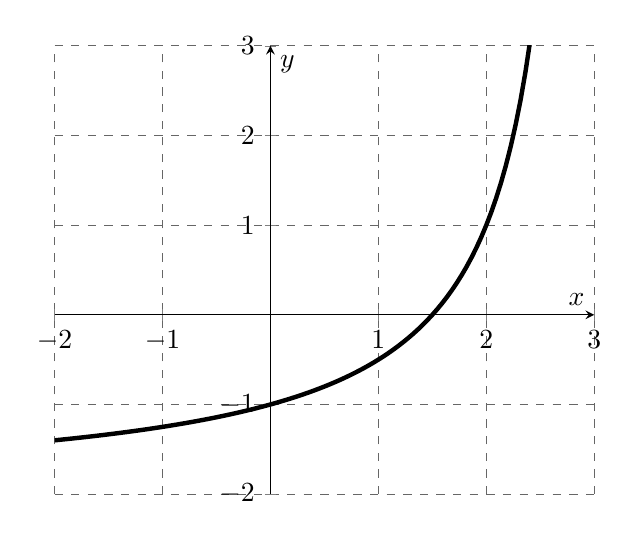
\begin{tikzpicture}
 \begin{axis}[
    xmin = -2, xmax = 3,
    ymin = -2, ymax = 3, xtick={-2,-1,...,3}, ytick={-2,-1,...,3},
    grid=both, grid style={ thin, black!60, dashed},axis x line=middle, axis y line=
middle, xlabel={$x$}, ylabel={$y$}]
    \addplot[ultra thick, ->,samples=100,
        domain = -2:2.5,
    ] {(x)/(3-x)-1};
    %\addplot[thick,->] coordinates {(-1,0) (6,0)};
\end{axis}
\end{tikzpicture}

Left is a sketch of the graph of\\ $\ds f(x)= \frac{x}{3-x} -1$. \\

\textbf{Sketch and label the tangent line} to the graph at the point $P = (2,1).$\\

\textbf{Sketch and label the secant line} between $P = (2,1)$ and $Q = (0,f(0)).$
\end{multicols}
\end{subproblems}
\newpage

\problem{5} A drone is descending vertically. Its height in meters,
$h$, is given by the expression $\ds
h(t) = 10 - \sqrt{t}$ where $t$ represents time in seconds. Find the
{\bf average velocity} of the drone between 1 second and 4
seconds. Include units in your answer.
\vfill

\problem{8} Evaluate the expressions below. Assume all angles are measured in radians. If an expression is undefined, write ``undefined''.\\


\begin{subproblems}
\begin{multicols}{2}
	\item $\displaystyle \sin ( \pi /4)= $
	\item $\displaystyle \cos (7 \pi /6)=$
\end{multicols}
\vspace{1in}	
\begin{multicols}{2}
	\item $\displaystyle \sec (\pi /3)= $
	\item $\displaystyle \tan (- \pi /2) =$
\end{multicols}
\vspace{1in}
\end{subproblems}


\problem{2} Use the right triangle below, with side lengths 12, 5, and 13,  to evaluate the expressions.\\

\vspace{.1in}

\begin{multicols}{2}
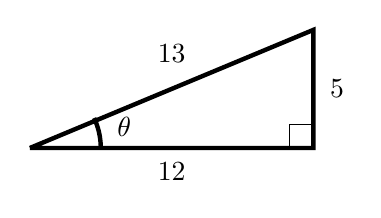
\begin{tikzpicture}[scale=0.3]
\draw[ultra thick] (0,0) -- (12,0) -- (12,5) -- (0,0);
\node at (6,-1){12}; 
\node at (13,2.5){5}; \node at (6,4){13};
\draw [ultra thick,domain=0:25] plot ({3*cos(\x)}, {3*sin(\x)});
\node at (4,.9){$\theta$};
\draw (11,0) -- (11,1) -- (12,1);
\end{tikzpicture}
\begin{subproblems}
\item $\displaystyle \cot (\theta) =$
\item $\displaystyle \csc (\theta) =$
\end{subproblems}
\end{multicols}
\vspace{.5in}


	
\end{document}
%%% Local Variables:
%%% mode: LaTeX
%%% TeX-master: t
%%% End:
